\documentclass[12pt,a4paper]{article}
\usepackage[margin=1in]{geometry}

\usepackage{polski}
\usepackage[utf8]{inputenc}

\usepackage{amsfonts}
\usepackage{amsthm}
\usepackage{enumerate}
\usepackage{graphicx}
\usepackage{hyperref}

\usepackage{indentfirst}

\author{Łukasz Bratos, Paweł Rubin}
\title{AlkoHurt - projekt bazy danych dla magazynu w hurtowni alkoholi}
\date{styczeń 2019}

\begin{document}
\maketitle

\section*{Cel projektu}

    Celem projektu jest stworzenie aplikacji bazodanowej pomagającej w zarządzaniu pojedynczym magazynem w hurtowni alkoholi. Aplikacja będzie oparta o relacyjną bazę danych z użyciem języka SQL.
    
\section*{Użytkownicy}
    
    Aplikacja będzie udostępniać dostęp do bazy danych z trzech poziomów: administratora, kierownika i pracownika. Każdy z nich posiada dedykowane uprawnienia:
    \begin{itemize}
        \item \textbf{Administrator} - dostęp do całej bazy danych
        \item \textbf{Kierownik} - dodawanie i aktualizowanie nowych produktów, dostaw oraz dostawców
        \item \textbf{Pracownik} - dodawanie nowych zamówień oraz klientów
    \end{itemize}
    
\section*{Baza danych}
\subsection*{Tabele}

    Baza danych będzie posiadała następujące tabele (dokładny schemat na  \hyperref[fig:diagram]{diagramie UML}):
    
    \begin{itemize}
        \item \textbf{users} - użytkownicy bazy danych (z podziałem na uprawnienia dostępu)
        \item \textbf{products} - informacje o cenie i ilości produktów
        \item \textbf{liquors} - szczegółowe informacje o alkoholach wysokoprocentowych
        \item \textbf{beers} - szczegółowe informacje o piwach
        \item \textbf{wines} - szczegółowe informacje o winach
        \item \textbf{supplies} - informacje o dostawach
        \item \textbf{supplies info} - dokładne informacje o konkretnej dostawie
        \item \textbf{suppliers} - informacje o dostawcach
        \item \textbf{sales} - informacje o sprzedażach (historycznych i planowanych)
        \item \textbf{sales info} - dokładne informacje o konkretnej sprzedaży
        \item \textbf{clients} - informacje o klientach
    \end{itemize}
    
\subsection*{Triggery}

    \begin{itemize}
        \item Trigger uruchamiany przed dodaniem nowego trunku - najpierw dodaje krotkę do tabeli \textbf{products}, a następnie odpowiednie krotki do właściwych tabel
        \item Trigger uruchamiany po aktualizacji tabel \textbf{sales} lub \textbf{supplies} - po zmianie wartości pola \textit{done} na \texttt{true} aktualizuje ilość produktów w tabeli \textbf{products}
    \end{itemize}        

\subsection*{Procedury}

    \subsubsection*{Administrator}
        \begin{itemize}
            \item \textsf{add\_user} - dodaje nowego użytkownika
        \end{itemize}

    \subsubsection*{Kierownik}
        \begin{itemize}
            \item \textsf{add\_liquor} - dodaje nowy alkohol wysokoprocentowy do bazy danych
            \item \textsf{add\_beer} - dodaje nowe piwo do bazy danych
            \item \textsf{add\_wine} - dodaje nowe wino do bazy danych
            \item \textsf{add\_supplier} - dodaje nowego dostawcę do bazy danych
        \end{itemize}
    
    \subsubsection*{Pracownik}
        \begin{itemize}
            \item \textsf{add\_client} - dodaje nowego klienta do bazy danych
            \item \textsf{plan\_supply} - dodaje nową planowaną dostawę
            \item \textsf{plan\_sale} - dodaje nową planowaną sprzedaż
            \item \textsf{show\_quantity} - pokazuje szacowaną dostępność danego towaru na dany dzień
            \item \textsf{update\_sale} - zmienia wartość pola \textit{done} na \texttt{true} w tabeli \textbf{sales}
            \item \textsf{update\_supply} - zmienia wartość pola \textit{done} na \texttt{true} w tabeli \textbf{supplies}
        \end{itemize}
        
        Ponadto użytkownik o wyższej hierarchii posiada dostęp do wszystkich procedur o niższym poziomie dostępu.
        
\subsection*{Diagram UML}
        
\begin{figure}
    \centering
    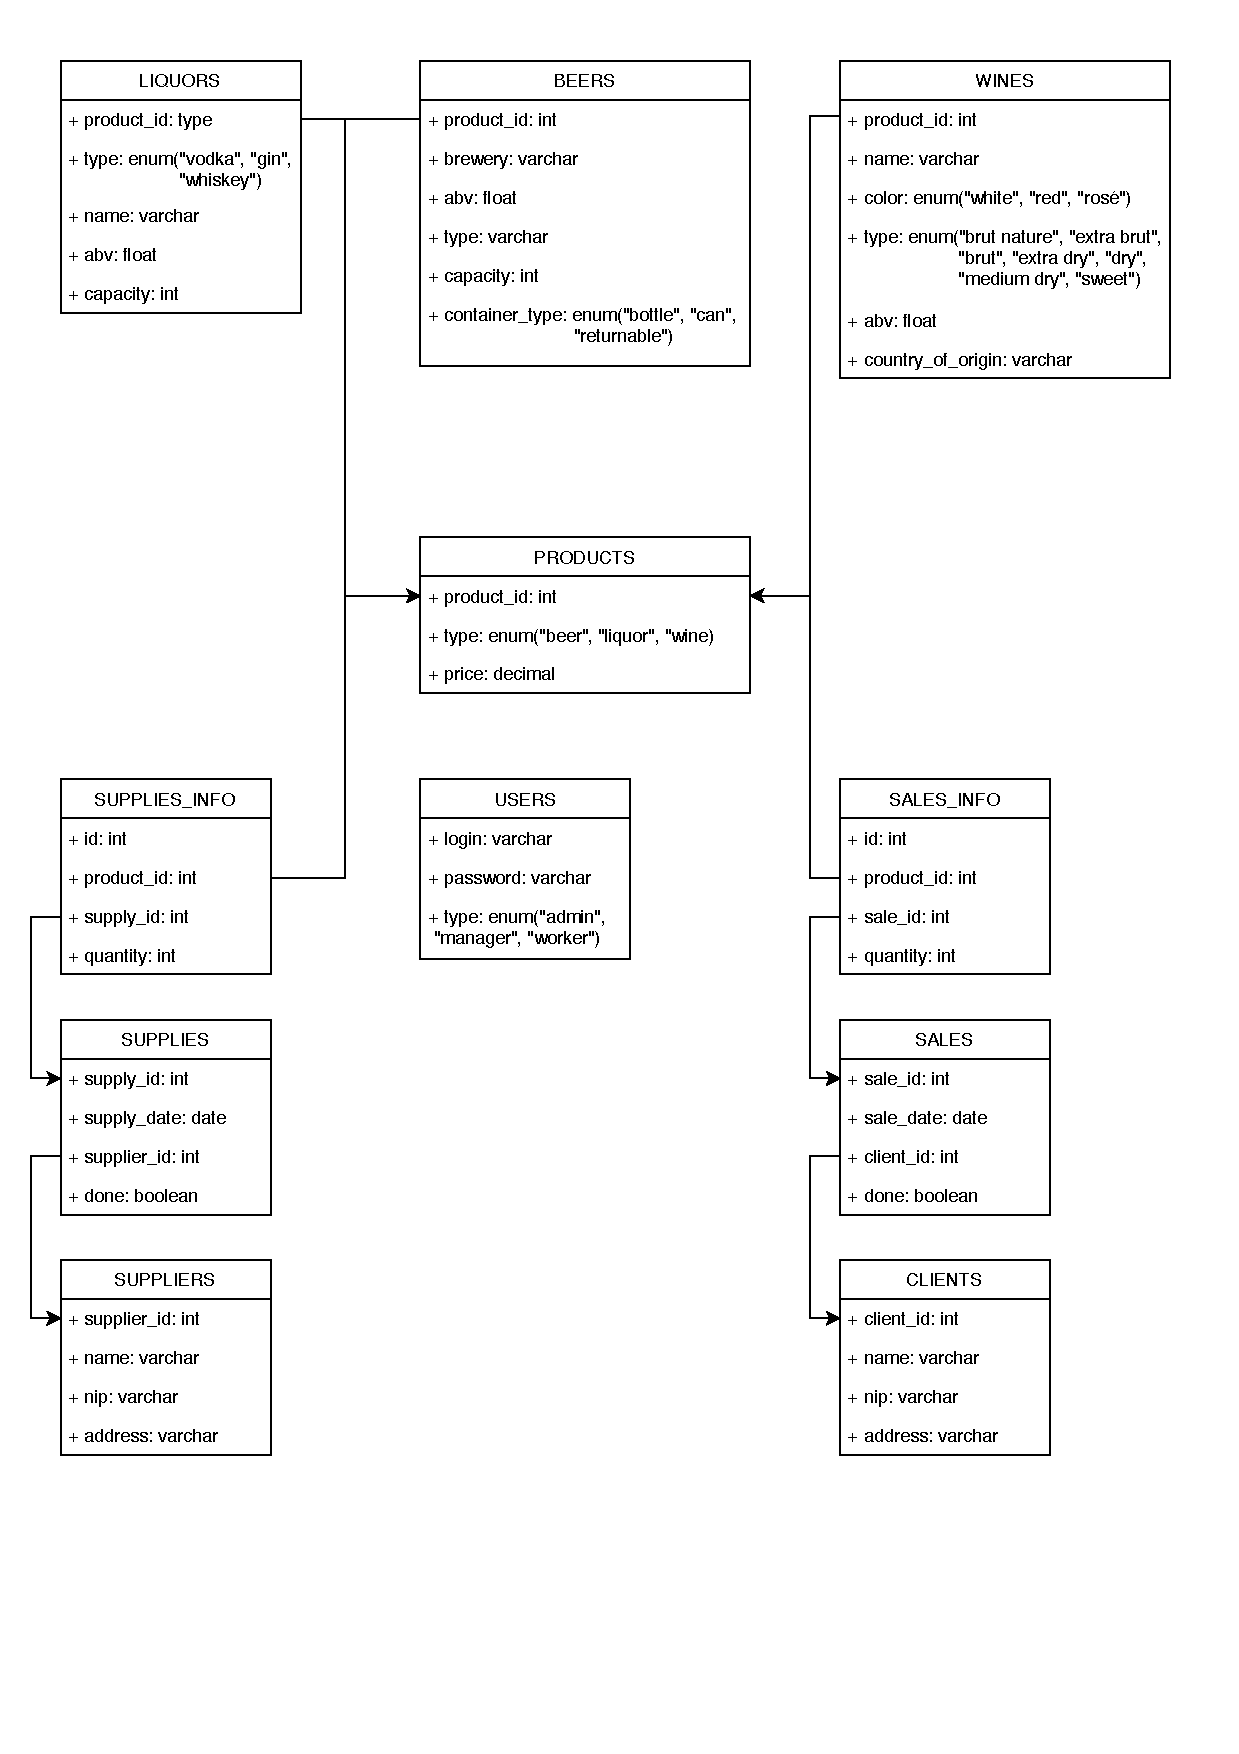
\includegraphics[width=\columnwidth]{uml}
    \caption{Diagram UML}
    \label{fig:diagram}
\end{figure}
    
    
\end{document}
